\documentclass[12pt]{article}
\usepackage{amsmath}
\usepackage{amsfonts}
\usepackage{geometry}
\usepackage{graphicx}
\usepackage{setspace}
\usepackage{parskip}
\usepackage{hyperref}
\usepackage{graphicx}


\geometry{a4paper, margin=1in}
\setstretch{1.2}

\title{Statistical Outlier Detection Notes}
\author{}
\date{}

\begin{document}

\maketitle

\section*{Outlier Detection Using Mean and Standard Deviation (Z-Score Based Outlier Detection)}

To detect outliers in a dataset $\Delta$, we use the mean and standard deviation:

\begin{itemize}
    \item $\mu(\Delta)$: Mean of the data
    \item $\sigma(\Delta)$: Standard deviation of the data
\end{itemize}

\subsection*{Normal Range}

The normal range is defined as:

\[
\mu(\Delta) \pm 2\sigma(\Delta)
\]

This means most data points (about 95\% if normally distributed) are expected to lie within this range.

\subsection*{Outlier Condition}

A value is considered an outlier if:

\[
\Delta < \mu(\Delta) - 2\sigma(\Delta) \quad \text{or} \quad \Delta > \mu(\Delta) + 2\sigma(\Delta)
\]


\begin{itemize}
    \item $\Delta$ - Orderbook Delta Depth of 5\% from Coinbase
    \item $\mu(\Delta)$ - Mean of $\Delta$
    \item $\sigma(\Delta)$ - Standard deviation of the dataset
\end{itemize}







\newpage


\subsection*{Idea behind}

\begin{itemize}
    \item This method assumes data is roughly normally distributed.
    \item Using $2\sigma$ captures approximately 95\% of data points under a normal distribution.
    \item You can adjust the multiplier (e.g., $3\sigma$) for stricter or looser thresholds.
\end{itemize}


\begin{figure}
    \centering
    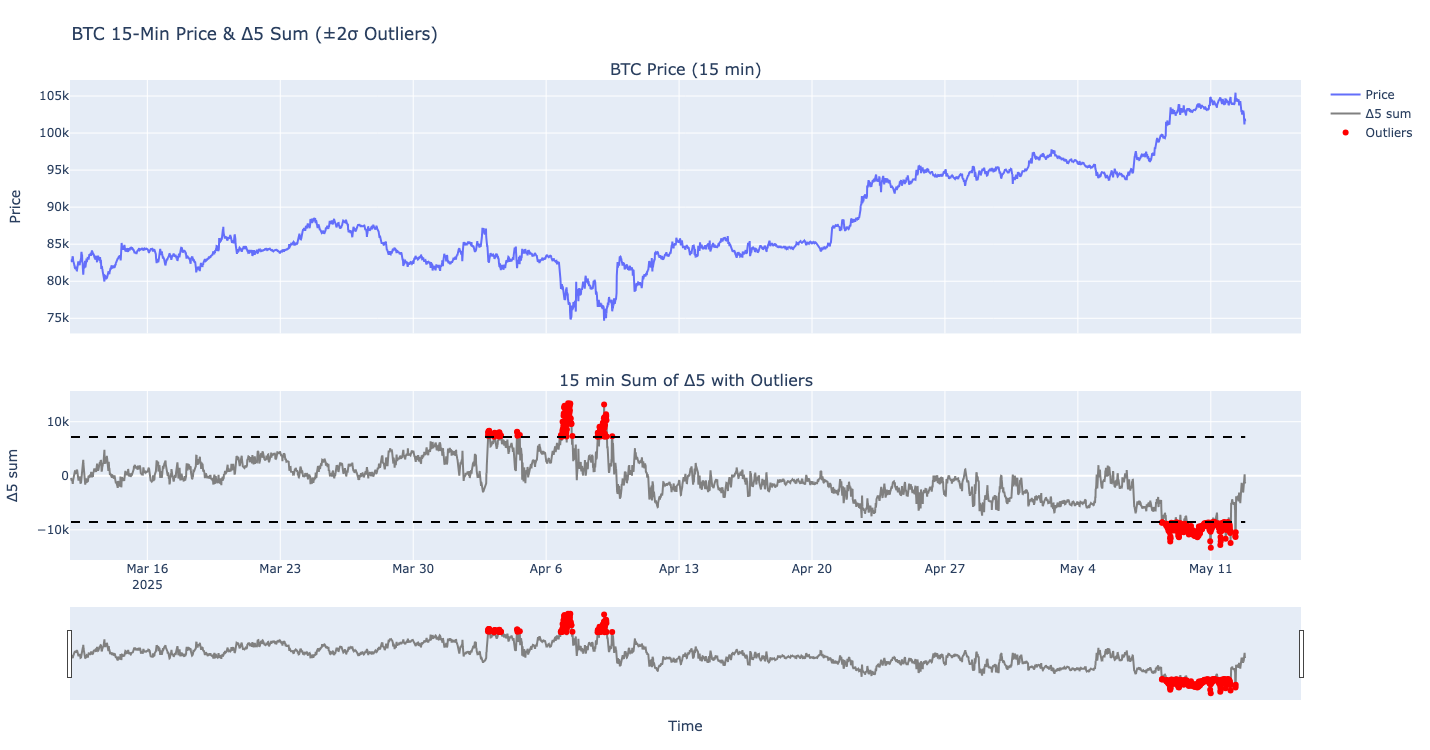
\includegraphics[width=1\textwidth]{imgs/ResultsOfSTDoutlierDecection.png}
    \caption{results over a two month data set}
\end{figure}


\subsection*{Future Plans}

\begin{itemize}
    \item Test on more data
    \item use rolling windows (e.g. 1 day or 1 week) for local context.
    \item Compare sensitivity with +- 1.5$\sigma$ or +-2.5$\sigma$
\end{itemize}


\section*{Orderbook Delta Based RSI}




\end{document}